In diesem abschließenden Kapitel möchten wir nun die in
\Cref{chap:implementation} beschriebene Realisierung von
\Cref{alg:primalDualIteration} mit Abbruchkriterium
\eqref{eq:terminationCriterion} im Solve-Schritt der AFEM-Schleife aus
\Cref{fig:afemLoop} an einigen Benchmark-Problemen untersuchen.
Dabei konstruieren wir Probleme, bei denen die exakte Lösung bekannt ist,
nach \Cref{sec:constructionInputSignal}. 
Als besonderes Augenemerk betrachten wir dabei zwei Eingangssignale.
Andere Funktionen werden wir bei Bedarf betrachten, um bestimmte Eigenschaften
zu untersuchen im Vergleich zu diesen beiden Benchmark-Problemen.
Für ein Experiment mit exakter Lösung betrachten wir zunächst auf $[0,\infty)$
für einen Parameter $\beta\geq 1/2$, wobei wir stets $\beta =1$ wählen, 
die Funktionen
\begin{align*}
  u_1(r)&\coloneqq
  \begin{cases}
    1, 
    & \text{falls } r\in \left[0,\frac{1}{6}\right],\\
    1+(6r-1)^\beta, 
    & \text{falls } r\in \left(\frac{1}{6}, \frac{1}{3}\right],\\
    2, 
    & \text{falls } r\in \left(\frac{1}{3}, \frac{1}{2}\right],\\
    2\left(\frac{5}{2}-3r\right)^\beta, 
    & \text{falls } r\in \left(\frac{1}{2}, \frac{5}{6}\right],\\
    0, 
    & \text{falls } r\in \left(\frac{5}{6}, \infty\right),\\
  \end{cases}\\
  \sgn\big(\partial_r u_1(r)\big) 
  &\coloneqq
  \begin{cases}
    12r-36r^2, 
    & \text{falls } r\in \left[0,\frac{1}{6}\right],\\
    1, 
    & \text{falls } r\in \left(\frac{1}{6}, \frac{1}{3}\right],\\
    \cos(\pi(6r-2)), 
    & \text{falls } r\in \left(\frac{1}{3}, \frac{1}{2}\right],\\
    -1, 
    & \text{falls } r\in \left(\frac{1}{2}, \frac{5}{6}\right],\\
    -\frac{1+\cos(\pi(6r-5))}{2}, 
    & \text{falls } r\in \left(\frac{5}{6}, \infty\right).
  \end{cases}
\end{align*}
Nach \Cref{eq:constructionInputSignal} ist $u$ mit dieser Wahl von
$\sgn\big(\partial_r u_1\big)$ die Lösung von \Cref{prob:continuousProblem} mit
Eingangssignal
\begin{align*}
  f_1(r)
  &=
  \begin{cases}
    \alpha-12(2-9r), 
    & \text{falls } r\in \left[0,\frac{1}{6}\right],\\
    \alpha\left(1+(6r-1)^\beta\right)-\frac{1}{r}, 
    & \text{falls } r\in \left(\frac{1}{6}, \frac{1}{3}\right],\\
    2\alpha+6\pi\sin(\pi(6r-2))-\frac{1}{r}\cos(\pi(6r-2)), 
    & \text{falls } r\in \left(\frac{1}{3}, \frac{1}{2}\right],\\
    2\alpha\left(\frac{5}{2}-3r\right)^\beta+\frac{1}{r},
    & \text{falls } r\in \left(\frac{1}{2}, \frac{5}{6}\right],\\
    -3\pi\sin(\pi(6r-5))+\frac{1+\cos(\pi(6r-5))}{2r}, 
    & \text{falls } r\in \left(\frac{5}{6}, \infty\right).
  \end{cases}
\end{align*}

\begin{figure}[!ht]
  \centering
  \begin{subfigure}[b]{.48\linewidth}
    \caption{$f_1$}
    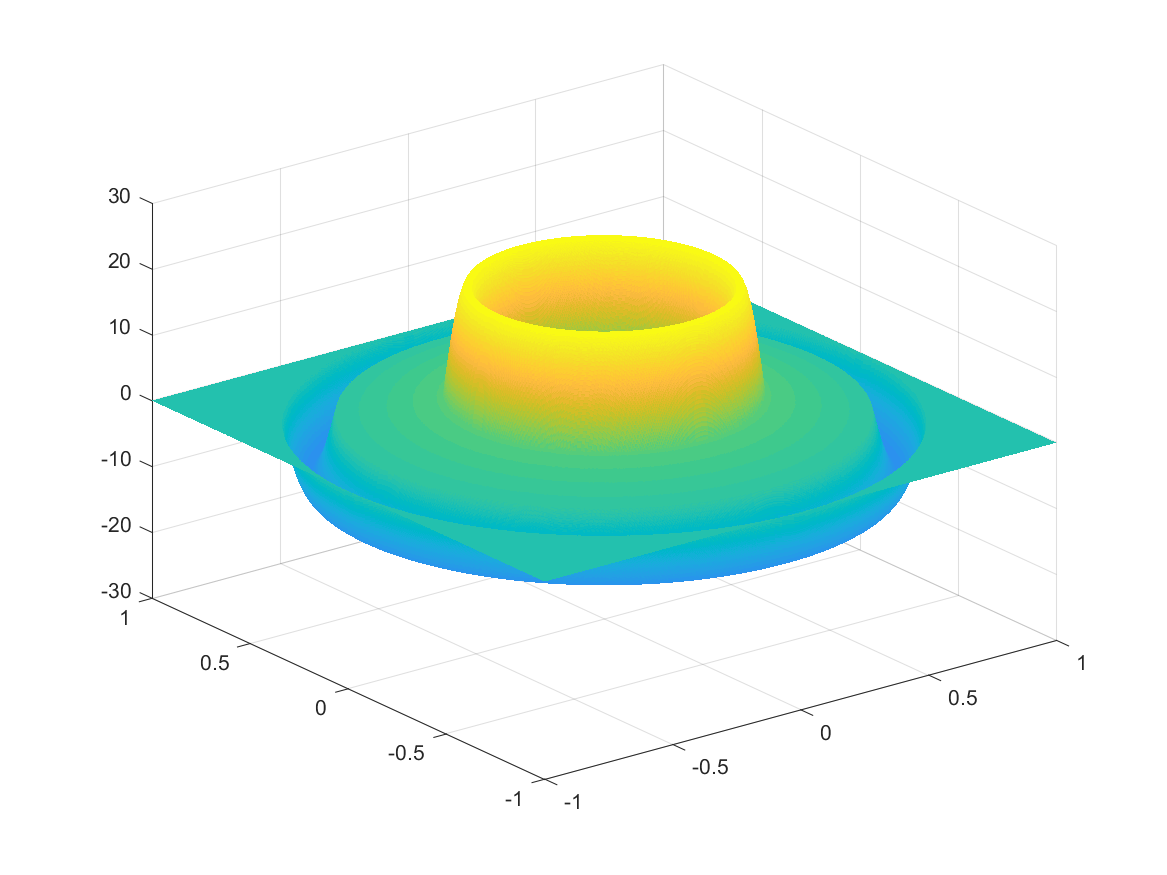
\includegraphics[trim = 40 30 30 30, clip, width=\linewidth]
      {pictures/chapExperiments/secGeneralInfo/f01Plots/inSi.png}
    \label{fig:f01InSi}
  \end{subfigure}
  \quad
  \begin{subfigure}[b]{.48\linewidth}
    \caption{$u_1$}
    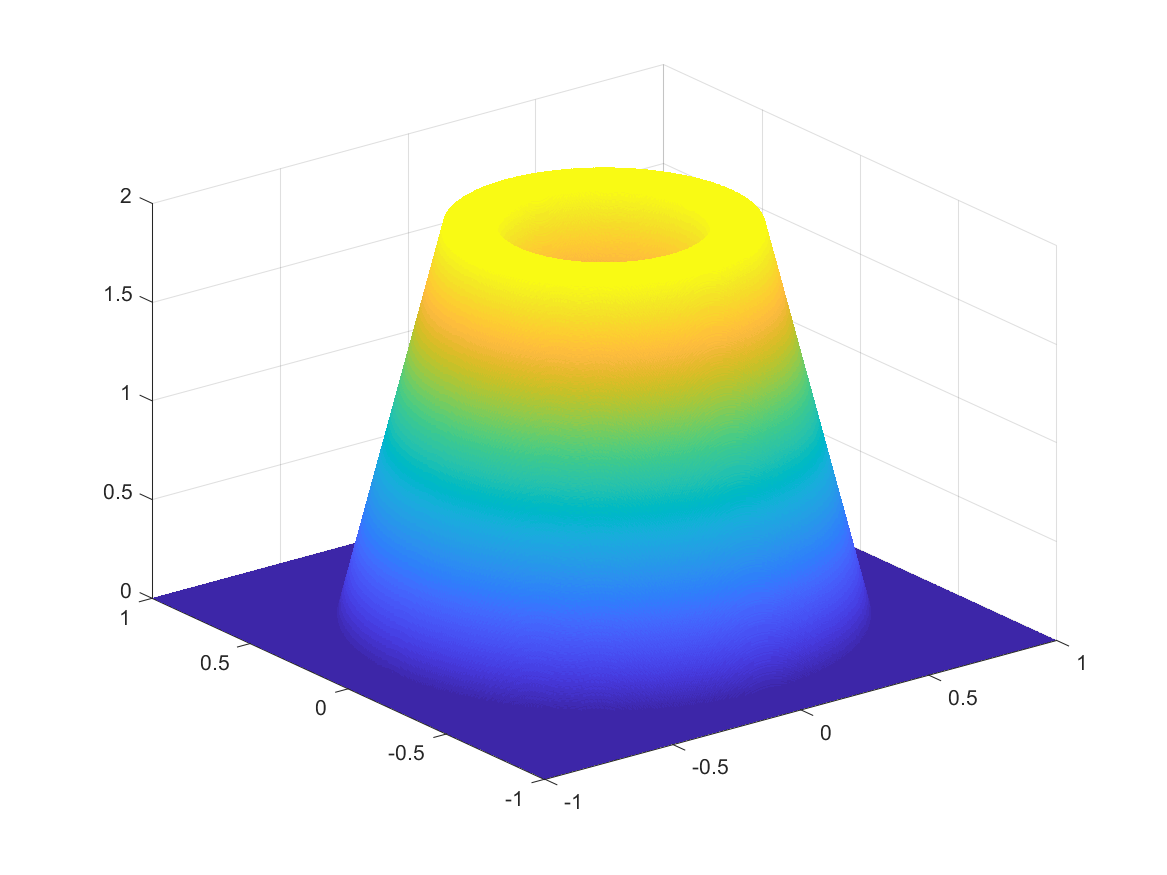
\includegraphics[trim = 40 30 30 30, clip, width=\linewidth]
      {pictures/chapExperiments/secGeneralInfo/f01Plots/exactSolution.png}
    \label{fig:f01ExactSol}
  \end{subfigure}

  \begin{subfigure}[b]{.48\linewidth}
    \caption{$f_1$ entlang der x- und y-Achse}
    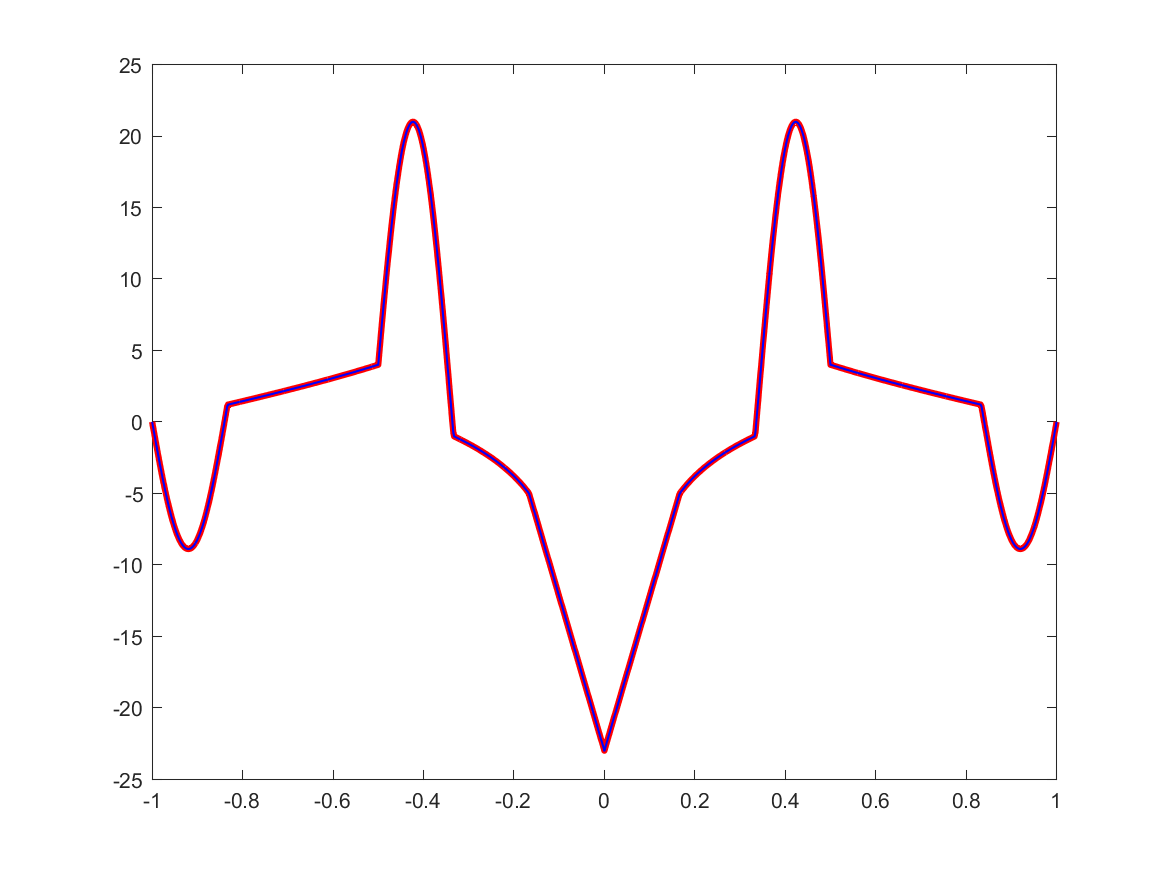
\includegraphics[trim = 50 30 50 20, clip, width=\linewidth]
      {pictures/chapExperiments/secGeneralInfo/f01Plots/inSiAxis.png}
    \label{fig:f01InSiAxis}
  \end{subfigure}
  \quad
  \begin{subfigure}[b]{.48\linewidth}
    \caption{$u_1$ entlang der x- und y-Achse}
    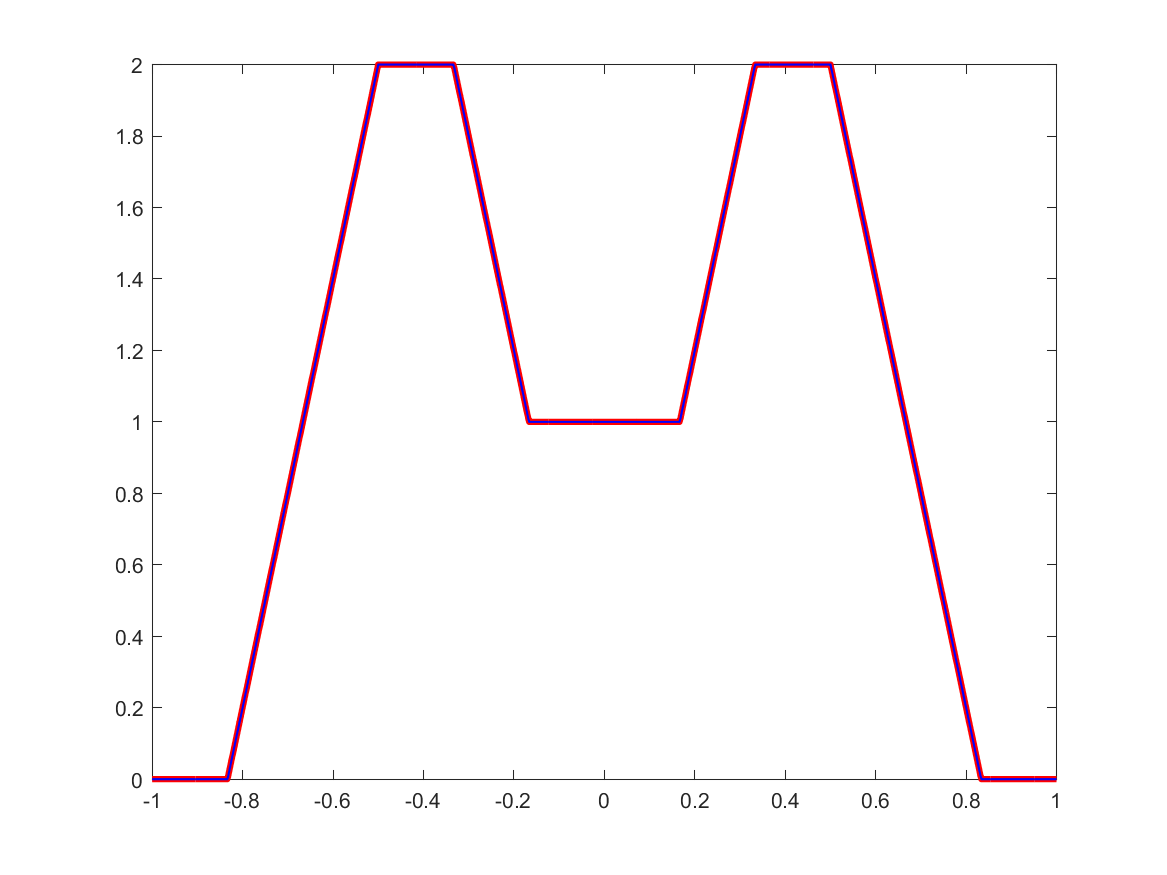
\includegraphics[trim = 50 30 50 20, clip, width=\linewidth]
      {pictures/chapExperiments/secGeneralInfo/f01Plots/exactSolutionAxis.png}
    \label{fig:f01ExactSolAxis}
  \end{subfigure} 
  \caption{Eingangssignal $f_1$ und exakte Lösung $u_1$ sowie deren
  Darstellungen entlang der x-Achse (blau) und der y-Achse (rot) für
  $\alpha=1$.}
  \label{fig:f01Plots}
\end{figure}

Ableitung von u wird zu Berechung von E(u) gebraucht nochmal sagen, sonst 
irrelevant für Experimt

vielleicht ,der Gradient von u ist\ldots, damit approximieren wir die
exakte Energie \ldots)

Nach \Cref{sec:constructionInputSignal} lauten die entsprechenden Ableitungen
\begin{align*}
  \partial_r f_1(r)
  &=
  \begin{cases}
    108,
    & \text{falls } r\in\left[0,\frac{1}{6}\right],\\
    6\alpha\beta(6r-1)^{\beta-1} +\frac{1}{r^2}, 
    & \text{falls } r\in\left(\frac{1}{6},\frac{1}{3}\right],\\
    \left(36\pi^2+\frac{1}{r^2}\right)\cos(\pi(6r-2))
    + \frac{6\pi}{r}\sin(\pi(6r-2)), 
    & \text{falls } r\in\left(\frac{1}{3},\frac{1}{2}\right],\\
    -\left(6\alpha\beta\left( \frac{5}{2}-3r \right)^{\beta-1}+
    \frac{1}{r^2}\right),
    & \text{falls } r\in\left(\frac{1}{2},\frac{5}{6}\right],\\
    -\left( \left( 18\pi^2+\frac{1}{2r^2} \right)\cos(\pi(6r-5))
    +\frac{1}{2r^2} + \frac{3\pi}{r}\sin(\pi(6r-5))\right), 
    &\text{falls } r\in\left(\frac{5}{6},\infty\right),
  \end{cases}\\
  \partial_r u_1(r) 
  &= 
  \begin{cases}
    0,
    & \text{falls } r\in\left[0,\frac{1}{6}\right],\\
    6\beta(6r-1)^{\beta-1}, 
    & \text{falls } r\in\left(\frac{1}{6},\frac{1}{3}\right],\\
    0, 
    & \text{falls } r\in\left(\frac{1}{3},\frac{1}{2}\right],\\
    -6\beta\left( \frac{5}{2}-3r \right)^{\beta-1},
    & \text{falls } r\in\left(\frac{1}{2},\frac{5}{6}\right],\\
    0,
    &\text{falls } r\in\left(\frac{5}{6},\infty\right).
  \end{cases}
\end{align*}



Ein Problem mit unstetigem Eingangssignal legen wir besonderes
Augenmerk auf das Graufarbenbild \texttt{cameraman} aus \cref{fig:cameraman}
als Eingangssignal. 

[nach cameraman Erwähnung] Auch für dieses Beispiel, das stark unregulär ist,
haben selbst deutlich höhere Integrationsgrade als 10 zu keinen veränderten
Raten geführt. 
Auch geringere nicht, da aber alle Methoden, die \texttt{integrate} aufrufen
werden vor oder nach der primalen-dualen Iteration aufgerufen, 
beeinflusst dies die Laufzeit nicht negativ und wird so gewählt um möglichst
exakte Integration zu gewährleisten.

==================

degree4Integrate FÜR UNSERE AUFRUFE VON INTEGRATE schreiben (denn errorCRL2
nutzt degree 12 immer, also wäre die aktuelle Formulierung falsch)
irgendwo sollte eh noch geschrieben werden ,,zur berechnung des Fehler wird
die Methode aus AFEM genutzt, die immer Grad 12 hat unabh von degree4Integrate
aus Tabelle ...)

Zwar können die Funktionen hier sehr unregulär sein
Für keines der Experimente wurde, auch mit deutlich höheren Wahlen von
degree4Integrate, andere Raten beobachtet.

integrate wird nie während der Iteration aufgerufen, ein relativ hoher 
Integrationsgrad beeinflusst die Laufzeit vernachlässigbar (das betonen,
dass Integrate nur außerhalb ausgeführt wird)

==================

Als initiale Geometrie nutzen wir dafür entsprechend immer
\texttt{BigSquare} des AFEM-Pakets (vlt. verweis auf Package falls vorhanden)
ohne initiale Rotverfeinerung [Abbildung mit der Triangilierung linken], da
diese den Einheitskreis enthält.
Fur dieses nutzen wir als initiale
Triangulierung für das erste Level des AFEM Algs die Triangulierung
\texttt{Square} [mach so wie eben] [s. Abb \ldots].

\begin{figure}[!ht]
  \centering
  \begin{subfigure}[b]{.48\linewidth}
    \caption{\texttt{BigSquare}}
    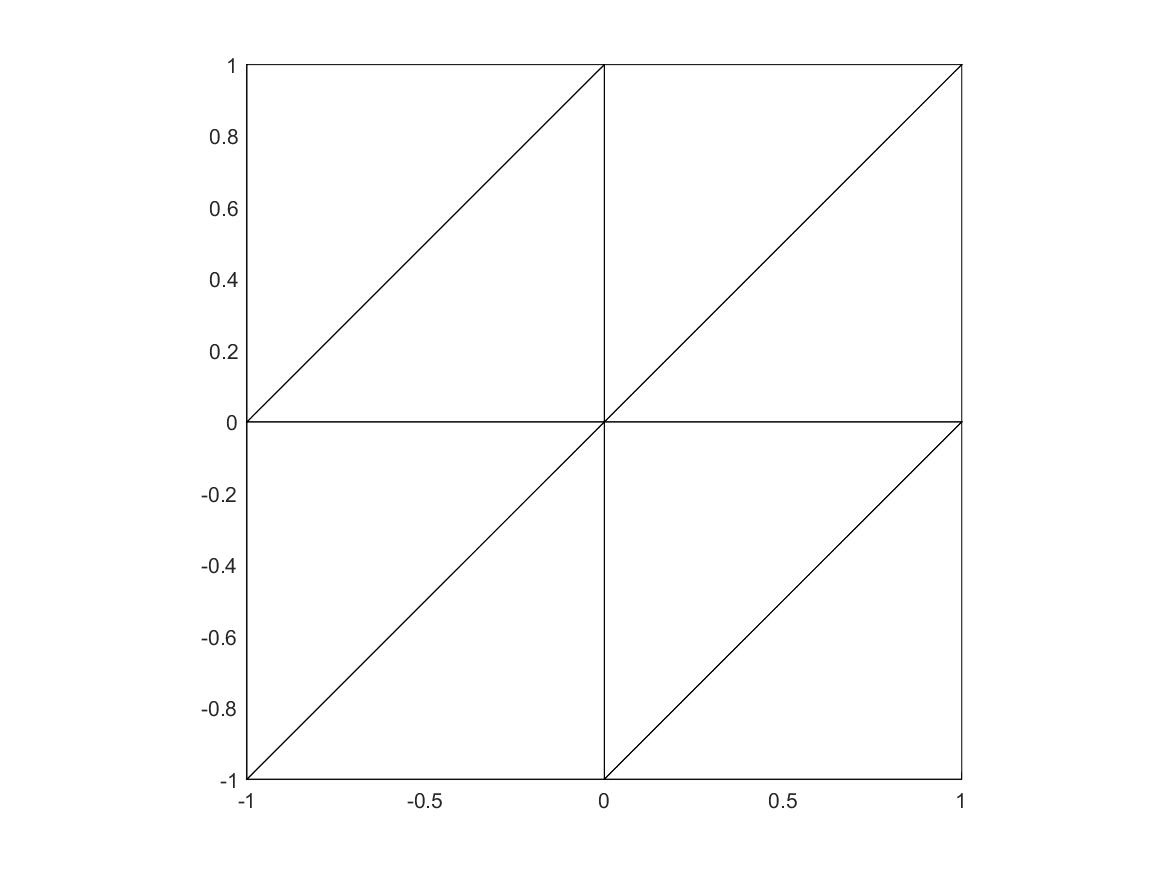
\includegraphics[trim = 90 30 90 20, clip, width=\linewidth]
      {pictures/chapExperiments/secGeneralInfo/bigSquareTriang.png}
    \label{fig:triangBigSquare}
  \end{subfigure}
  \quad
  \begin{subfigure}[b]{.48\linewidth}
    \caption{\texttt{Square}}
    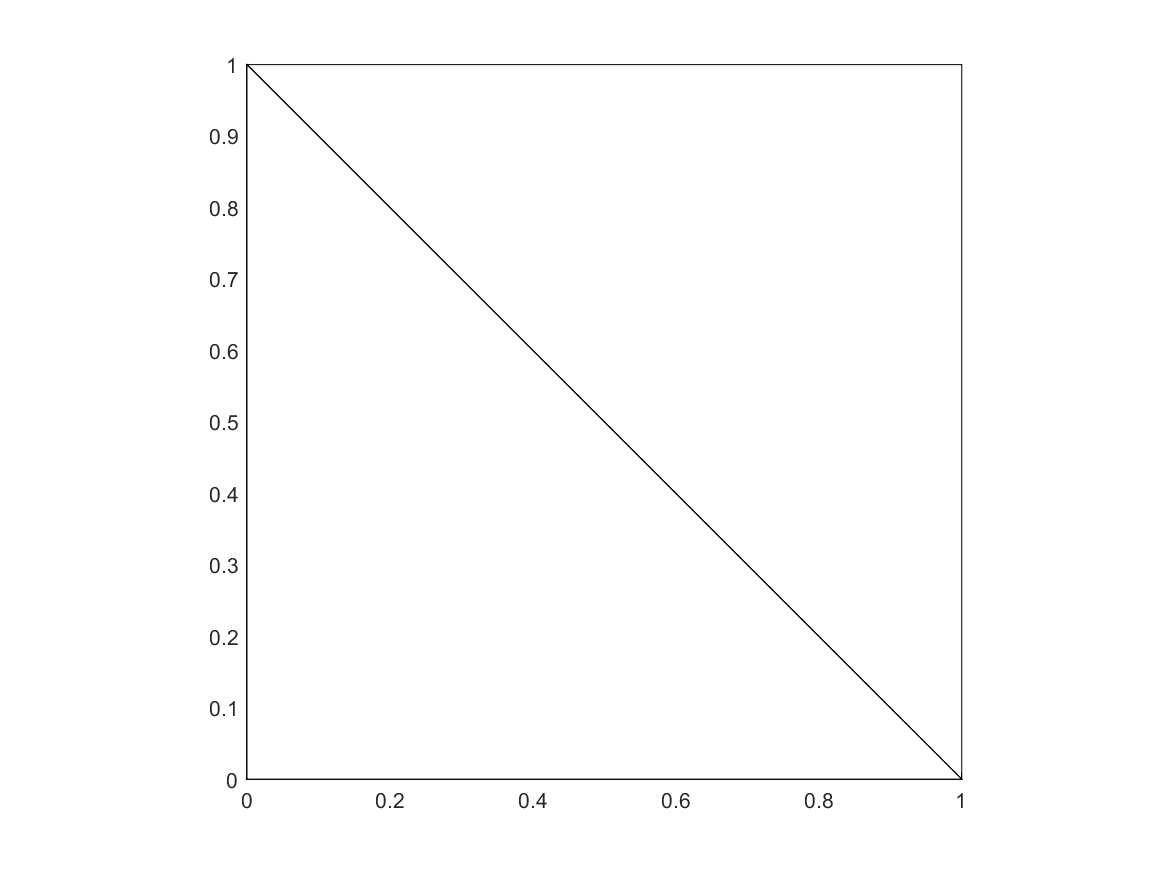
\includegraphics[trim = 90 30 90 20, clip, width=\linewidth]
      {pictures/chapExperiments/secGeneralInfo/squareTriang.png}
    \label{fig:triangSquare}
  \end{subfigure}
  \caption{In den Experimenten genutzte initiale Triangulierung.}
  \label{fig:initialTriangulations}
\end{figure}

Führen wir eines der Experimente mit adaptiver Netzverfeinerung durch, so
wählen wir den Bulk-Parameter für den Mark-Schritt des AFEM-Algorithmus, soweit
nicht anders angegeben, $\theta=0.5$.
Auf die Wahl der Parameter $\tau$ und $\epsstop$ für die primale-duale
Iteration werden wir im folgenden Abschnitt [ref] eingehen.
Zur Wahl des Parameters $\gamma$ auf dem Verfeinerungsindikator betrachten
wir in Abschnitt (Experimente mit exakter Lösung) ein.

  überlegen, welche Parmeter für jedes Experiment nochmal gesagt werden sollen
  definitiv: 


\section{Wahl der Parameter für die primale-duale Iteration}
alles zu tau mit hypothesse

bei tau, argumentiere, das 1e6 Iterationen ausreichen (vgl mit tau = 1, sage, 
wie viele tau = 1 gebraucht hat) Sage, dass man theoretisch ausrechnen kann,
wenn initialer Fehler etc bekannt ist, wie viele Iteration benötigt werden (da 
die Fehler ja konstant bleiben und 1e6 mal aufaddiert wurden muss das 
Thm schief gehen irgendwann)

==================

  - s. gleich, Effekt von großen/kleinen alpha bzw. tau entsprechend ein
    paar Experiment mit gleicher Lösung machen und gleichem Input (was alpha
    irgendwie disqualifiziert, oder?) (vlt gucken ob Raten oder so in corr
    einzeichnenbar sind)

kleine tau und alpha nicht groß lässt die energie nur osszilierend von oben
konvergieren (s. Ordner) (auch tau = h/10 oder so ähnlich (bartels))
wird alpha zu kleinen tau groß gewählt, behebt dass den Effekt.
Die obere Schranke der Summe im Beweis ist c/(tau*alpha), d.h. die Schranke
ist für z.B. alpha=1 und tau=1/100 schon relativ groß, wahrscheinlich größer
als 100
kann das das verhalten erklären?
falls ja, wäre dann tau = 1 nicht die ideale Wahl?
das wäre dann eine Section in Experimenten wert, die das vermutet und dann per
Experimenten überprüft, ob tau=1 besser ist als tau=1/100 etc
Gleiches für die Wahl von alpha (nur das alpha noch mehr Anwendung dahinter hat),
aber große alpha sollten für die Iteration besser sein als kleine 

==================

beispiel ohne konvergenz aufzeigen und dafür auch die Triangulierung zeigen

==================

zu abbruchkriterium

  - wähle bei epsStop 1e-2, 1e-3 und 1e-4 und sage, dass bei 1e-4 der Effekt 
    in den Freiheitsgraden die wir rechnen noch nicht auftritt und es deshalb
    so gewählt wird

2) Größe von epsStop: dokumentieren, dass z.B. bei $10^{-2}$ der Fehler irgendwann
nicht mehr fällt und damit die Wahl $10^{-4}$ (ca.) begründen.
Ein Plot, in denen der $L^2$ Fehler (und/oder Fehler der Energien) verglichen wird
(untersuchen, ob es da qualitative Unterschiede gibt zwischen -3, -4, -5, ...)

3) $|||.||| ~ h^{-1} ||.||$ korrekt? Enc stetig bzgl Konvergenz in L2 (Zsmh. 
   zwischen eNc und bar12sqrt)
   (discrete Poincare (bar15, Lem 3.7), inverse Ungleichung (bar15, Lem. 3.5)),
   Bsp. Lvl13 in $f01eps10^{-4}$ hat hMin ~ $10^{-3}$, Graphen sehen korrekt
   verschoben aus


1) terminatin Criteria Vergleich (f01Term und camTerm)
    - eNcAbsDiff wegen Oszillation ungeeignet (da das mal 'zu früh') die 
      Toleranz erreichen kann obwohl es noch nicht soweit ist
    - die anderen sind alle gleich gut, oder? ist die Höhe der Graphen relevant?
      (natürlich müsste man epsStop analog kleiner wählen, wenn man z.B. den
      parallel und niedrigeren bar15TerminationWithoutL2 wählt)

==================

zu gamma (0, 0.5, 1) noch irgendwo ein Experiment mit Info, dass 0 und 1e-4 oder
so was identisch sind

  - gamma = 0 im Vergleich der gammas mit erwähnen (da es sich von gamma 1e-4
    nicht unterscheider visuell (nochmal prüfen ob das stimmt) nur eines der
    beiden gammas plotten und genau diese Info in einem Satz erwähnen und vlt
    auch in der Legende beides für einen Graphen angeben gamma = 0, 1e-4)


\section{Experimente mit bekannter exakter Lösung}

f01 vor allem

==================

gucke in der Arbeit ob $S^1(\Tcal)$ jemals nochmal genutzt wird. Falls nicht,
die Definition der Couran-Finite-Elemente-Funktionen verschieben aus Notation
in die Einleitung an die Stelle, an der ich über Bartels Ansatz schreibe

insbesondere auch die Quelle dann einfach da erwähnen

wird wohl in der Auswertung erwähnt für die Rate von Bartels, also kann 
voraussichtlich bleiben

==================

  - f01 mit großem alpha konvergiert am Anfang preasymptotisch schnell aber
    scheint bei großen Freiheitsgraden dann auch die Rate 1/2 (für Gleb Kram)
    bzw. 1/4 oder so für Fehler anzunehmen (also gleiche Raten wie alpha=1).
    liegt daran, dass für große alpha die Werte anfangs explodieren und damit
    die Konvergenz rapide ist (auch die Iterationen sind viel kürzer, hier
    lohnt sich sicherlich auch der Vergleich der misc plots und nochmal verweis
    auf die Abschätzung aus Konvergenzbeweis (großes alpha, womöglich weniger
    Iteration))

==================

  - Section Name: Convergence of energies (see Bar12, do some experiment
    chapter like that)

  - energy during iteration doesn't strictly converge from above to some value
    for small tau (e.g. 1/100)

==================

hier vielleicht auch einmal einwerfen, wie die Iteration konvergiert
(vlt auch in der vorigen Section, im Vergleich zu den schlechten Wahlen,
die dort auch getroffen werden.

==================

dann abschweif zu höhere Regularität

  - h20 Beispeil genau so wie H10, also das vielleicht nur erwähnen ,,eine 
    noch stärke Regularitätsannahme im Beispeil f04, bei dem Lsg und f H20 sind,
    verbesserte die Raten nicht weiter (verschiebt nur die Graphen nach unter,
    d.h. früher kleiner Fehler)

==================

hier eventuell auch experimte für AFEM Params?

==================

dann insgesamt raten abarbeiten und interpretieren


\section{Graufarbenbilder als Eingangssignale}
cameraman

==================

abschweif zu denoise example aus intro hier erklären

==================

zum abschluss zu approximation von white circle mit stetigeer funktion (plots
dementsprechend

  - circle stuff, etas sind vergleichbar (was gut, weil so erwarte)


\section{Fazit und Ausblick}

AUSBLICK (vielleicht in die Arbeit schreiben)
  
  Randdaten verallgemeinern
    nochmal aufschreiben wo CR10 angenommen wird und eventuell darauf verweisen 
    im Ausblick (bis dahin notieren welche Funktionen und in welchem Maß)
    (in solvePrimalDualFormulation zum Erstellen der rechten Seite)
    
  Bartels Code anpassen und vergleicen

%%%%% hiervor finalized
%%%%% ab hier Skizze

Dazu gehört ein Beispiel mit bekannter Lösung, das wir nach cite(section)
konstruieren, ein komplexes Beispiel ohne Lösung mit einer unstetigen Funktion,
hier ein Bild als Eingangssignal und eine einfache, diskontinuierliche Funktion
als Eingangssignal und eine, ebenfalls nach section konstruierte stetige 
Approximation dieser.

\todo[inline]{Neue Gliederung: vgl Storn oder noch besser Sophie, statt
Auswertung ,Zusammenfassung und Ausblick'. Oder einfach wie Franz, ohne
Zsmfssg, ,Numerische Experimente und SChlussfolgerung' oder so}


Alle Allgemeinen Infos unter die Hauptüberschrift, keine eigene Section,
da auch integrate gleich 10 erwähnen



Mache alle mögliche Sachen, prüfe Dinge die gelten sollen. Für ein
Beispiel (z.B. CCs) fange mit basics an, also mal an einem Iterationsplot
aufzeigen, dass die Energie tatsächlich von oben gegen was konvergiert und 
gehe dann weiter zu anderen Themen wie den Raten, GLEB etc.

\todo[inline]{Probiere auch thm:convexity irgendwie informell zu erwähnen ,,wir
sehen, dass sogar ohne die Sprünge das stimmt\ldots`` oder so}

\todo[inline]{in chap 6 cf.s auf integrate etc nicht ständig sonder einmal 
gesammelt am Anfang oder drauf achten, dass das nur beim ersten Erwähnen zitiert 
wird}

\todo[inline]{Programm gibt Sprungtermsumme aus, z.B. stagnierend bei 11 auf
allen Leveln, darauf vielleicht noch kurz in der Auswertung eingehen ,man
sieht, dass die Sprünge tatsächlch im nonkonformen Problem nicht minimiert
werden oder so'}




Zuerst allgemeines, alle Infromationen, die ggf bei allen Experimten in den 
folgenden Abschnitten immer gleich sind und möglicherweise kurze Kommentare,
warum diese entspreched gewählt sind.

\bigskip

Alle Experimentparameter die stets gleich gesetzt sind Eingangs einmal erwähnen,
insbesondere degree4Integrate, was immer als 10 gesetzt wird, mit ähnlichem 
Kommentar wie PB auf S 30


\bigskip

Bei Beschreibung wie die Bilder der Einleitung zur Rauschunterdrückung
entstanden sind auch erwähnen, dass $f=\alpha g$ eine Rolle spiele usw.


%%%%%%%%%%%%%%%%%%%%%%%%%%%%%%%%%%%%%%%%%%%%%%%%%%%%%%
\todo[inline]{Beschreibe hier nur das allgemeine Vorgehen und die 
mathematischen Hintergründe und schreibe die genutzten Beispiele an
entsprechender Stelle in Numerische Beispiele oder so. Die ungenutzten Beispiele 
die trotzdem im Ordner liegen können in einem extra Abschnitt aufgezählt werden}
Schema ist dann: Nach section Konstruktion einer exakten Lösung erhalten wir
für die Wahl u mit sgn bla die rechte Seite f.
Die Details bei bestimmten Konstruktionen, etwa ,,um H2 zu erhalten fordern wir
noch`` ergänzen beim Vorstellen des entsprechenden Experimentes, hier nur das 
allgemeinste, das, was CC wirklich geschrieben hat.
%%%%%%%%%%%%%%%%%%%%%%%%%%%%%%%%%%%%%%%%%%%%%%%%%%%%%%
Wir wollen damit Experimente konstruieren um Aussagen in \ldots oder \ldots
zu prüfen, entsprechend müssen wir noch fordern
Da in den Kapiteln GLEB und bla u in H10 relevant wird, fordern wir
weiterhin \ldots
%%%%%%%%%%%%%%%%%%%%%%%%%%%%%%%%%%%%%%%%%%%%%%%%%%%%%%


Für die Funktion
\begin{align*}
  u_2(r)\coloneqq 
  \begin{cases}
    1, & \text{wenn } 0\leq r\leq\frac{1-\beta}{2},\\
    -\frac{1}{\beta}r + \frac{1+\beta}{2\beta}, & 
    \text{wenn } \frac{1-\beta}{2}\leq r\leq \frac{1+\beta}{2},\\
    0, & \text{wenn } \frac{1+\beta}{2}\leq r,
  \end{cases}
\end{align*}
erhält man mit der Wahl
\begin{align*}
  \sgn&(\partial_r u_2(r)) \\
  &\coloneqq 
  \begin{cases}
    \frac{4}{1-\beta}r\left(\frac{1}{1-\beta}r -1\right), &
    \text{wenn } 0\leq r\leq\frac{1-\beta}{2},\\
    -1, & \text{wenn } \frac{1-\beta}{2}\leq r\leq \frac{1+\beta}{2},\\
    \frac{4}{(\beta-1)^3}
    \left( 4r^3-3(\beta+3)r^2 +6(\beta+1)r-3\beta-1\right), & 
    \text{wenn } \frac{1+\beta}{2}\leq r\leq 1,
  \end{cases}
\end{align*}
die rechte Seite
\begin{align*}
  f_2(r)\coloneqq 
  \begin{cases}
    \alpha - \frac{4}{1-\beta}\left(\frac{3}{1-\beta}r - 2\right), &
    \text{wenn } 0\leq r\leq\frac{1-\beta}{2},\\
    -\frac{\alpha}{\beta}\left( r-\frac{1+\beta}{2} \right) +\frac{1}{r}, & 
    \text{wenn } \frac{1-\beta}{2}\leq r\leq \frac{1+\beta}{2},\\
    \frac{-4}{(\beta-1)^3}
    \left( 16r^2 -9(\beta+3)r + 12(\beta+1) - \frac{3\beta+1}{r}\right), & 
    \text{wenn } \frac{1+\beta}{2}\leq r\leq 1.
  \end{cases}
\end{align*}

Es folgen zwei Beispiele mit exakter Lösung $u_3=u_4 \in H^2_0((0,1)^2)$, 
gegeben durch 
\begin{align*}
  u_3(r)=u_4(r)\coloneqq 
  \begin{cases}
    1, & \text{wenn } 0\leq r\leq\frac{1}{3},\\
    54r^3 - 81r^2 + 36r - 4, & 
    \text{wenn } \frac{1}{3}\leq r\leq \frac{2}{3},\\
    0, & \text{wenn } \frac{2}{3}\leq r.
  \end{cases}
\end{align*}
Mit der Wahl
\begin{align*}
  \sgn&(\partial_r u_3(r)) \\
  &\coloneqq 
  \begin{cases}
    54r^3-27r^2, & \text{wenn } 0\leq r\leq\frac{1}{3},\\
    -1, & \text{wenn } \frac{1}{3}\leq r\leq \frac{2}{3},\\
    -54r^3 + 135r^2 - 108r + 27, & \text{wenn } \frac{2}{3}\leq r\leq 1,
  \end{cases}
\end{align*}
erhalten wir die rechte Seite
\begin{align*}
  f_3(r)\coloneqq 
  \begin{cases}
    \alpha - 216r^2 + 81r, &
    \text{wenn } 0\leq r\leq\frac{1}{3},\\
    \alpha\left(54r^3 - 81r^2 + 36r - 4\right)) + \frac{1}{r}, & 
    \text{wenn } \frac{1}{3}\leq r\leq \frac{2}{3},\\
    216r^2 - 405r + 216 - \frac{27}{r}, & 
    \text{wenn } \frac{2}{3}\leq r\leq 1,
  \end{cases}
\end{align*}
für die gilt $f_3\in H^1_0$
und mit der Wahl
\begin{align*}
  \sgn&(\partial_r u_4(r)) \\
  &\coloneqq 
  \begin{cases}
    -1458r^5 + 1215r^4 - 270r^3, & \text{wenn } 0\leq r\leq\frac{1}{3},\\
    -1, & \text{wenn } \frac{1}{3}\leq r\leq \frac{2}{3},\\
    -243r^4 + 756r^3 - 864r^2 + 432r - 81, 
    & \text{wenn } \frac{2}{3}\leq r\leq 1,
  \end{cases}
\end{align*}
erhalten wir die rechte Seite
\begin{align*}
  f_4(r)\coloneqq 
  \begin{cases}
    \alpha + 8748r^4 - 6075r^3 + 1080r^2, &
    \text{wenn } 0\leq r\leq\frac{1}{3},\\
    \alpha\left(54r^3 - 81r^2 + 36r - 4\right) + \frac{1}{r}, & 
    \text{wenn } \frac{1}{3}\leq r\leq \frac{2}{3},\\
    1215r^3 - 3024r^2 + 2592r - 864 + \frac{81}{r}, & 
    \text{wenn } \frac{2}{3}\leq r\leq 1,
  \end{cases}
\end{align*}
für die gilt $f_4\in H^2_0$.


\begin{align*}
  \partial_r f_2(r) &= 
  \begin{cases}
    -\frac{12}{(1-\beta)^2},&\text{wenn }0\leq r\leq\frac{1-\beta}{2},\\
    -\frac{\alpha}{\beta}-\frac{1}{r^2},&
    \text{wenn } \frac{1-\beta}{2}\leq r\leq \frac{1+\beta}{2},\\
    -\frac{4}{(1-\beta)^3}\left( 32r-9(\beta+3)+\frac{3\beta+1}{r^2} \right),&
    \text{wenn } \frac{1+\beta}{2}\leq r\leq 1,\\
  \end{cases}\\
  \partial_r u_2(r) &= 
  \begin{cases}
    0,&\text{wenn }0\leq r\leq\frac{1-\beta}{2},\\
    -\frac{1}{\beta},&
    \text{wenn } \frac{1-\beta}{2}\leq r\leq \frac{1+\beta}{2},\\
    0,&\text{wenn } \frac{1+\beta}{2}\leq r,
  \end{cases}\\
  \partial_r f_3(r) &=
  \begin{cases}
    - 432r + 81, & \text{wenn } 0\leq r\leq\frac{1}{3},\\
    \alpha\left(162r^2 - 162r + 36\right) - \frac{1}{r^2}, & 
    \text{wenn } \frac{1}{3}\leq r\leq \frac{2}{3},\\
    432r - 405 + \frac{27}{r^2}, & 
    \text{wenn } \frac{2}{3}\leq r\leq 1,
  \end{cases}\\
  \partial_r f_4(r) &=
  \begin{cases}
    34992r^3 - 18225r^2 + 2160r, & \text{wenn } 0\leq r\leq\frac{1}{3},\\
    \alpha\left(162r^2 - 162r + 36\right) - \frac{1}{r^2}, & 
    \text{wenn } \frac{1}{3}\leq r\leq \frac{2}{3},\\
    3645r^2 - 6048r + 2592 - 864 - \frac{81}{r^2}, & 
    \text{wenn } \frac{2}{3}\leq r\leq 1,
  \end{cases}\\
  \partial_r u_{3,4}(r) &=
  \begin{cases}
    0, & \text{wenn } 0\leq r\leq\frac{1}{3},\\
    162r^2 - 162r + 36, & 
    \text{wenn } \frac{1}{3}\leq r\leq \frac{2}{3},\\
    0, & \text{wenn } \frac{2}{3}\leq r\leq 1,
  \end{cases}\\
\end{align*}

====================
aus altem Auswertungen.tex (neues: s. Storn, Puttkams)

In diesen Abschnitt werten wir die in \Cref{chap:experiments} erhaltenen
Ergebnisse aus.

\todo[inline]{folgendes weniger ausführlich einbringen, wohl
auch eher im Auswertungskapitel ,,in Bartels wird in
citeEntsprechendesLemma die garantierte Rate für \ldots bewiesen. In unseren
Experimenten \ldots}

Zunächst betrachten wir \cite[S. 309, Theorem 10.7]{Bar15}. Diese
Abschätzung kontrolliert den
$L^2$-Fehler zwischen den Minimierern $u_\C\in S^1(\Tcal)$ und
$u\in\BV(\Omega)\cap L^2(\Omega)$ des Funktionals $I$ aus \Cref{eq:rofModel} in
den entsprechenden Räumen. Obwohl wir eine andere Formulierung des ROF-Modells 
betrachten und sich insbesondere das Funktional $\Enc$ aus unserer diskreten,
nichtkonformen Formulierung von $I$ unterscheidet, ähneln sich die 
Probleme möglicherweise genug, um die folgende Rate für unsere Formulierungen
experimentell feststellen zu können.

\begin{theorem}
  \label{thm:errorEstimateCourant}
  Sei $\Omega\subset\Rbb^2$ sternförmig und $g\in L^\infty(\Omega)$.  Seien
  weiterhin $u\in\BV(\Omega)\cap L^2(\Omega)$ und $u_\C\in S^1(\Tcal)$ die
  Minimierer des Funktionals $I$ aus \Cref{eq:rofModel} in den entsprechenden
  Räumen.

  Dann existiert eine Konstante $c\in\Rbb_+$, sodass
  \begin{align*}
    \frac{\alpha}{2}\Vert u-u_\C\Vert^2\leq
    ch^{1/2}.
  \end{align*}
\end{theorem}

====================

Punkte auf die bei den Auswertungen eingegangen werden sollte

Raten

Verfeinerungsindikator

Fazit und Ausblick
